\section{DNN}\label{chapter-ML-section-XGB}

\fullcite{DNN}

\subsection{Neurons}

\begin{center}
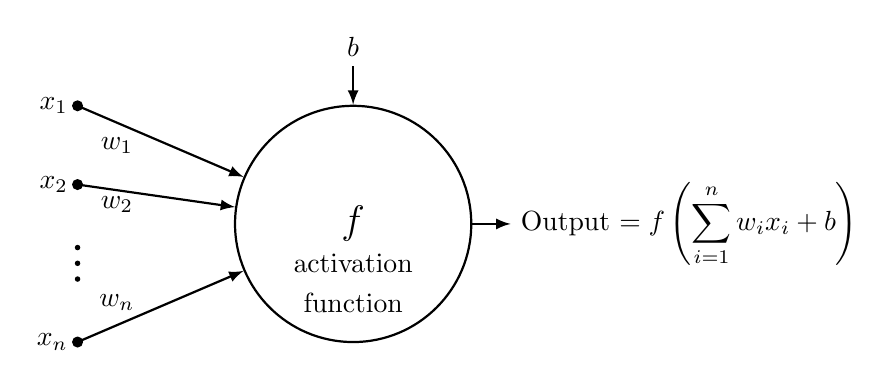
\begin{tikzpicture}

\node [draw, thick, circle, minimum size = 3 cm] (N) at (0,0) {};

\foreach \yi/\N in {1.5/1,0.5/2,-1.5/n}{
\fill (-3.5,\yi) circle(2pt) node [left] {$x_{\N}$};
\draw [thick, -latex] (-3.5,\yi) -- (N);
}

\draw (-3,1) node {$w_1$};
\draw (-3,0.25) node {$w_2$};
\draw (-3,-1) node {$w_n$};

\foreach \x/\y in {-3.5/-.5}{
\fill (\x,\y) circle (1pt);
\fill (\x,\y+.2) circle (1pt);
\fill (\x,\y-.2) circle (1pt);
}

\draw [thick, latex-] (N) -- (0,2) node [above] {$b$};

\draw [thick, -latex] (N) -- (2,0) node (output) [right] {Output $\displaystyle = f\left(\sum_{i=1}^n w_ix_i + b\right)$};

\draw (0,0) node {\Large $f$};
\draw (0,-.5) node {activation};
\draw (0,-1) node {function};

\end{tikzpicture}
\end{center}

Activation functions:
tanh, sigmoïd mostly for classification,
linear, relu, elu, selu, softmax, softplus ...

\subsection{Neural networks}

\newcommand{\drawN}[2][c]{
\node [draw, circle] (#1) at (#2) {};
}

\def\linkN#1#2{
\draw [-latex] (#1) -- (#2);
}

\begin{center}
\begin{tikzpicture}

\foreach \y in {0,1,2,-2}{
\foreach \x in {1,2,...,5}{
\drawN[\x\y]{\x,\y}
}
}

\foreach \yi/\N in {1.5/1,0.5/2,-1.5/n}{
\fill (-.5,\yi) circle(2pt) node [left] {$x_{\N}$};
\foreach \y in {0,1,2,-2}{
\draw [-latex] (-.5,\yi) -- (1\y);
}
}

\drawN[No]{6.5,0}

\draw [-latex] (No) --+ (.5,0) node [right] {$y=F(\vec{x})$};

\foreach \ya in {0,1,2,-2}{
\foreach \yb in {0,1,2,-2}{
\linkN{5\ya}{No}
\foreach \xa/\xb in {1/2,2/3,3/4,4/5}{
\linkN{\xa\ya}{\xb\yb}
}
}
}

\fill[white] (2.33,-2.5) rectangle (4.66,2.5);

\foreach \x/\y in {-.5/-.5,1/-1,2/-1,5/-1}{
\fill (\x,\y) circle (1pt);
\fill (\x,\y+.2) circle (1pt);
\fill (\x,\y-.2) circle (1pt);
}

\foreach \y in {0,1,2,-2}{
\fill (3.5,\y) circle (1pt);
\fill (3.5+.2,\y) circle (1pt);
\fill (3.5-.2,\y) circle (1pt);
}

\foreach \x in {.25,5.75}{
\draw [thick, dotted, CERNblue] (\x,-2.5) -- (\x,2.5);
}

\draw [CERNblue] (-.65, 2.5) node {Input layer\vphantom{Àq}};
\draw [CERNblue] (3, 2.5) node {Hidden layers\vphantom{Àq}};
\draw [CERNblue] (7.5, 2.5) node {Output layer\vphantom{Àq}};

\draw [thick, ltcolorred, latex-latex] (.25,-2.25) -- (5.75,-2.25);
\draw [ltcolorred] (3, -2.5) node {$N_L$\vphantom{Àq}};

\draw [thick, ltcolorred, latex-latex] (4.5,-2.125) -- (4.5,2.125);
\draw [ltcolorred] (4.5, 0) node [left] {$N_N$\vphantom{Àq}};

\end{tikzpicture}
\end{center}

\subsection{Training}
\subsubsection{Loss function}
loss == objective


= 0 when prediction == truth

minimize it!

\subsubsection{Optimizer and weights init}

Adam, Adadelta, SGD

parameters to optimize = weights and biais

need to init: (Glorot) uniform/normal

Glorot :  X. Glorot and Y. Bengio, “Understanding the difficulty of training deep feedforward neural networks”, in Proceedings of the thirteenth international conference on artificial intelligence and statistics, p. 249. 2010.


